\chapter{Best practices}\label{ch:best}
As an IoT application is designed as illustrated in figure \ref{fig:best0}, the development of an IoT application is split on two sides:
\begin{enumerate}
	\item IoT side - The part of the application that deals with sensors, devices and handles the communication between them and the main server.
	\item Client side - The part of the application that allows the final user to control the application.
\end{enumerate}


	\begin{figure}
	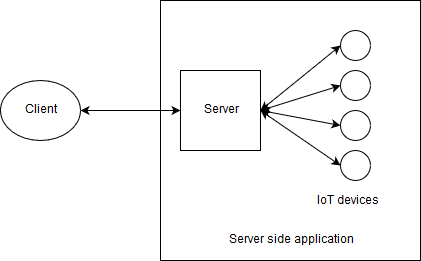
\includegraphics[width=\linewidth]{bestpractice-img0.png}
	\caption{One possible architecture of an IoT application.}
	\label{fig:best0}
\end{figure}

In order to develop a secure IoT application we must work on both sides; we have seen, in the previous chapter, how to attack and secure the communication between IoT devices and the main server, but we have not talked about the client side.\newline

The client side of an IoT application can be developed in different way, from a web application to a stand-alone application for Desktop or smartphone.\newline
From my experience in the company, the client side is developed as a web application in order to make it available both on desktop and smartphone without the need of developing two different application.\newline
It is important to highlight that each side must be treated with care, in fact it is useless to focus only on one side and left the other completely insecure; an attacker will exploit the weak ring to compromise your application, so the overall security of your system is equal to the weak ring security.\newline
Basically, the same effort must be done on both sides of the application.\newline

In this section, we will list down and discuss the best practice that you should follow in order to write secure IoT application from the client side point of view.\newline
I want to highlight that these best practices can be applied in all application development, they are not strictly related with IoT, that is because some section of an application, like for instance: password handling are present in lots of application that may have little in common to the IoT world.\newline
I will provide code to support my discussion where possible; if the use of code is not easy, we will use pseudo-code instead.\newline

\section{Never trust the client}
During the development of a client/server architecture, communications between the two parts is essential, but in order to develop a bulletproof application it is important to check always data received by the server.\newline

In order to have an example in mind we will refer to the classic web application model where the client side runs on a browser like Mozilla Firefox or Google Chrome, and where the server side application is written in PhP or similar languages.\newline

Even if we develop the client, the server must performs a check of the data received; the client may be used by a malicious user or the attacker may send data to our server without the aid of the client application with tools like cUrl, Postman or Telnet.\newline

Basically, when the server receives some data, before performing any operation it must:
\begin{enumerate}
	\item Authenticate the user if required.
	\item Check if the data is conform to your business application rules.
	\item If the data provided are used in a query, sanitize them with proper function.
	\item If the user is authenticated, check if he has the privilege to execute the operation requested.
	\item Send back the result if necessary.
\end{enumerate}

Now we will discuss in the details the five points.\newline

\begin{enumerate}
	\item	Most of the time, in order to provide a service or to allow the user to perform a certain action on our web application we want to authenticate the user, but sometimes this is not true, for instance: when a user does not have an account for our application we want to provide him a way to sign in, in this particular case we are allowing a user to execute an operation without authentication, just because he does not have login credential; note that the sign in of a user is a very critical point in your application, we will discuss about it in another best practice.
	\item At this point we want to check if the data received from the user are conform to what we expect, for instance if we expect to receive a short comment limited to 260 character, we must check that the provided comment does not exceed the limit; if we are dealing with file uploaded from a user it is extremely important to check if the provided file is not a malicious one, for instance suppose that we receive an image from the user, simple control like checking the extension of a file is absolutely a bad idea, in fact the extension of a file can be changed, thus it is possible to save a malicious executable program as a .png and upload it to a remote server, a better way to check that the image uploaded is really an image is checking the magic number also known as the file signature, data used to identify or verify the content of a file.
	Note that each type of data may need particular care, file are more complex to check instead of raw data like strings or integers; the suggestion is to study in details how to sanitize the particular data you are handling.
	\item In order to avoid SQL Injection, data loss and data leak, it is important to always sanitize a data used as a parameter for a query, a SQL Injection may drop the entire DB, or could silently leak information like username or password hash (I hope you do not have password saved as plain text). Now days is quite trivial to avoid these kind of attack with the aid of prepared statement which allows us to bind parameters in query in a very safe way.
	In general, prepared statement are supported by DB library of every important programming language and most of the case can be handled nicely with them.
	Anyway there are case where using a prepared statement is infeasible, if you want to allow a user to write down a query and execute it, using a prepared statement is difficult or even impossible, so you need to manually check the provided query.
	These warnings are valid even for NoSQL system, in this particular case there are no standard like for SQL system, so it may be more difficult to avoid them considering that there are no standard techniques.
	\item It is important to check the privilege associated to a user because we do not want everyone to execute operations that may change drastically our server application or even destroy it; without proper control, even the user with lowest privilege may execute operation reserved only to user with high privilege such as an administrator.
	Basically, what we need to do is placing an if statement where we check the user’s privilege before the critical operation, of course the user’s privilege is a data taken from your DB or other verified source, so the privilege level is something that is not sent from the client in order to avoid easy privilege escalation.
	\item There is nothing to say about this point.
\end{enumerate}

The golden rule is: never trust the client.

\section{Always check data from the server}
As we have seen, a server must not trust input from a client and it must sanitize them before using them, from the point of view of a client could seems strange to doubt about the server, but in reality the client must treat with care data received from the server because it could be a corrupted server or even a fake server.\newline
The scenarios are the following:
\begin{itemize}
	\item An attacker has taken control of the server and uses it to send malicious data.
	\item A DNS server has been corrupted by an attacker, when a client tries to obtain the address of the legitimate server, is redirected to
	a corrupted server.
\end{itemize}

The first is more realistic because a custom server may have more flaws that could be exploited, while a DNS server has been tested for years and is managed by Internet provider which we assume (and hope) have high security standard.\newline
Let us see a flaw in a web application.

\begin{lstlisting}[language=html]
//page.html
<html>
	<meta charset="UTF-8">
	<head><title>Test</title></head>
	<body>
		<div id=”placer”></div>
		<script scr=”vuln.js”></script>
	</body>
</html>
\end{lstlisting}

\begin{lstlisting}
//vuln.js
var req=new XMLHttpRequest();
req.onreadystatechange=function(){
	if(this.readyState==4 && this.status==200){
		var placer=document.getElementById(“placer”);
		placer.innerHtml=this.responseText;
	}
};
req.open(“GET”,”malicious.php”,true);
req.send();
\end{lstlisting}

\begin{lstlisting}[language=php]
//malicious.php
<?php
	echo “<img src=1 hidden onerror=alert('VULNERABLE!')>”;
?>
\end{lstlisting}

The client side code is composed by an html webpage and a JavaScript code that perform an AJAX request to the \texttt{malicious.php} page on the server.\newline
\textbf{Note:} in this case we choosed to use an AJAX request for simplicity, but nothing forbids us from using a WebSocket.\newline
While the server simply sends back a string, but this string contains JavaScript code.\newline
The problem here is that the client, in order to show the data received from the server, to the final user copies the content of \texttt{responseText} in the \texttt{innerHtml} of the \texttt{div} with \texttt{id=”placer”}.
In this particular case the data expected to be text, in reality is an html image tag containing JavaScript code for error handling (the image will never load), this code is added to the DOM and the code executed.\newline
In this case the code is a simple alert and does nothing to harm the client, but in a real scenario the malicious script will not be something so simple.\newline
The main problem here is that the client assumed that the data was safe and copied it to the innerHtml of a DOM element without sanitizing it.\newline

The \texttt{innerHtml} attribute of a DOM element is an easy way to add content to a web page, but it is also the easiest way to introduce vulnerabilities in your page.
In order to avoid such a trivial exploit it is recommended to sanitize the input before placing it on the DOM.\newline

On the internet, you can find this nice piece of code to sanitize a string:
\begin{lstlisting}
	function sanitize(var content){
	var elem=document.createElement(“div”);
	elem.innerHTML=content;
	return elem.innerText;
	}
\end{lstlisting}


The problem about this function is that it does not provide any security, so always check what you copy and paste in your code; it does not mean that what claimed is really what the code does.\newline
There are libraries around the web that provide function to sanitize string, one of the most famous is surely jQuery, it also offer other features but the \texttt{html()} function is great to avoid unwanted code execution when you need to place data on the DOM.\newline
This could be the structure of a correct handling of data received from the server.\newline
\begin{lstlisting}
var placer=document.getElementById(“placer”);
var sanitized=realSanitize(this.responseText);
placer.innerHtml=sanitized;
//aggiungere riferimento
\end{lstlisting}
The easy way to sanitize string is to rely on well-known libraries, but if for some reason you could not use them, the solution is to write your own sanitation function that will likely use regular expression, but be careful because it could be more difficult than expected and error prone, so test your code with care before using it in a release environment.\newline

\section{Password handling}
Password handling is a very critical section of every application, passwords are sensible data that must be treated carefully at different level, we will analyze how to handle password from the code and database perspective.\newline

\subsection{Handling password in code}
A password must be handled in a special way, in lots of code you can find snippet like the following:
\begin{lstlisting}[language=java]
String username=”user0”;
String password=”mypass0”;

login(username,password);
\end{lstlisting}

The real problem here is that the password is handled as a String, in high level languages like Java or C\#, strings are immutable, this means that a string cannot be modified in any way, so even if we change the reference in this way:
\begin{lstlisting}[language=java]
password=””;
\end{lstlisting}

We are not erasing the previous password content, we are changing the reference of the variable \texttt{password}, so the previous data are somewhere in memory, and it will be overwritten only when the garbage collector mark the area of memory as free and a new data is allocated in this particular area.\newline
If an attacker can dump the process or perform cold boot attack, he can steal login credential and other sensible data.
It is important to highlight that if an attacker can perform the previous operation you also have to deal with the fact that your system is vulnerable and compromised in some ways, or that the machine where the program runs is accessible to malicious users.\newline
In order to avoid data leak, we want to reduce the exposure of sensible data in our application as much as possible.\newline
In order to overwrite a password, we need a data structure that allows this operation, the easy way is to use an array of character instead of a string just in the way we deal with string in low-level languages like C.\newline
So, the previous snippet of code change in this way:
\begin{lstlisting}[language=Java]
String username=”user0”;
char[] password={‘m’,’y’,’p’,’a’,’s’,’s’,’0’};

login(username,password);
\end{lstlisting}


The main drawback of using an array of character is that is not comfortable, it obliges us to write code a bit more complex, and we do not have access to the utility function of the string class.
When the password is no more needed in our code we need to erase the content of the password, this could be done easily with this utility function:
\begin{lstlisting}[language=Java]
	public void destroy(char[] arr){
		for(int i=0;i<arr.length;i++)arr[i]=’0’;
	}
\end{lstlisting}

Always remember to erase the data when it is no more needed, otherwise all the work done to secure the password handling is wasted.\newline
\textbf{Note:} when you are dealing with a password, it is likely that you want to hash or encrypt it, most of the times cryptographic libraries deals with array of byte, converting an array of char to an array of byte is trivial so designing your system with this knowledge in mind could help you.\newline
Also remember that if you convert an array of character to an array of byte, the previous one is no more needed so erase its content and deal with the second one until you have finished your task, and remember to erase even this one.\newline
Basically, what we are trying to do is limiting the exposure of sensible data in memory as much as possible; of course if an attacker dump the process when the password is exposed there is no way to avoid the leak, but with this little trick we can make the task more difficult.\newline
Sometimes it may not be possible handle a password in this way for lots of different reason.\newline
For example in high level scripting language like JavaScript the primitive type char does not even exists, there is no easy way to handle a password without a string, you may think to handle it like an array of numbers, but it may be an overkill.\newline
Another example is the bad design of a library, suppose that you buy an API that require a login and the signature of the login function is the following:
\begin{lstlisting}
void login(String usr, String pwd);
\end{lstlisting}

In situation like that, there is nothing we can do, we cannot edit the signature and we must adapt our code in order to provide a String to the function.\newline
Handling the password like a character array is meaningless if you then need to convert it to a String.\newline

In C\# there is a special object called \texttt{SecureString} it provides a way to deal with password in a secure way, the content of a string is created via insert of single character, and the content of the string is encrypted in memory.\newline
It seems like a great way to deal with password but some of the API of C\# that requires a password as argument expect a String, so the utility of this object is not so high, also note that it does not provide any access to the content of the string (and sooner or later we will need to use the content), the only way to access it is to convert the \texttt{SecureString} object to a String with the aid of the static method \texttt{SecureStringToGlobalAllocUnicode(…)} of the \texttt{Marshal} class, which returns a \texttt{IntPtr} that can be converted in a \texttt{String} with the static method \texttt{PtrToStringUni(…)} of the \texttt{Marshal} class, but doing that simply throws away all the effort made in order to secure the password in memory considering that we are dealing again with a \texttt{String}.\newline

\subsection{Handling password in database}
Passwords are, most of the times, stored in a database; we are not interested in specifying which one because what we are about to say is valid for every system.\newline
The first thing we want to highlight is: do not store password as plain text in your database.\newline
If you store password as plaintext in your database, and an attacker steal your data, you are allowing access to your system freely.\\

Suppose that you are dealing with an e-commerce website, if an attacker could access as the user X it is likely it will be allowed to buy items with the credit card of X, or even steal the credit card number.\\
This will translate in problem and hassle for the user and an even big problem for you, and we have not even talked about the damage of image for your company, if the affair become of public domain (and it will, sooner or later).\\
In order to store password in a secure way we need three ingredients:
\begin{enumerate}
	\item A cryptographic hash function or a key derivation function.
	\item A salt generated from secure pseudo-random number generator.
	\item Number of iteration.
\end{enumerate}

A cryptographic hash function is a special hash function that map data of arbitrary size to a bit string of fixed size, designed to be one-way, in other word a function that is infeasible to invert.\\
A key derivation function is a cryptographic function that derive a secret key from a secret value such as a password.\\
The main difference between the two is that a key derivation function has a randomness property that is absent in a cryptographic hash function.\\
From now on, we will refer to both with the term hash function in order to make our exposure a bit more clear.\\
A salt is a sequence of random bit used together with the password as input for the hash function, when we say random we are referring to value generated with secure pseudo-random number generator, the common random number generator provided by all the standard library of programming languages are not appropriate for this kind of task.\\
The number of iteration is simply the number of time a particular hash function is executed in order to produce the output, we will talk about it in details in a few moments.\\

Storing a password as hash is recommended because if someone steal your database, it may be capable of reading the users’ records, on the other hand he will not be able to login because the password is not stored as plain text but as hash.\\
The login procedure (server side) takes a plain text password, calculates the hash from it and compares it with the one stored in the database; if the two hashes are the same, then the access to system is granted, otherwise it is not.\\
In other words, the only way to access the system with the credential of another user is to steal them with social engineering’s technique, guessing it with a dictionary attack or cracking it with a brute force attack.\\
Note that if an attacker has access to the database he can find users with the same password hash, this means that different users have the same password, so stealing the password of user1 means stealing also the password of user2.\\
If an attacker has stolen a database and crack the password of user X, it could be that the user X use the same password for different services, so if the attacker is able to break one hash he could gain the access even to other system, in this case is not only a fault from the development team but also from the users that used the same password.\\
There are also brute force attack that are particularly efficient because they work with large pre-computed hash table known as rainbow table; in order to avoid this attack we need to introduce a salt in order to make the use these table useless.
To avoid this kind of attack we are adding a random value known as salt in order to produce a different output every time the hash function is executed with the same password as input.\\
The salt is a value that must be saved with the hash, otherwise we will not be able to produce again the hash that match the one saved on the database.\\
It is not mandatory to maintain the salt secret, it can be saved in the database, or it can be saved separately.\\
With the aid of salt, we can make useless the use of a rainbow table because the attacker must know the salt, only after that he knows it can start a brute force attack that may takes a lot time if the password is not trivial.\\

It is also important to iterate the hash function a certain number of time in order to slow down the cracking attempt of an attacker.\\
First of all if the number of iteration is not known, the attacker must try all the password and hash them $n$ times, where $n$ is the number of iteration he has esteemed, so he must try blindly.\\
The number of attempts can be saved on the users’ record without problem, of course if an attacker steal your database he will know the value of $n$, but if all the precaution are applied he basically has no way to try a brute force attack that will takes lot of time.\\
It is important to design your system in a way that allow to customize the number of iteration during the years, that is because the computational power increases every year, so if a number of iteration $m$ was safe two years ago, it may be insecure nowadays, if you design your application in a good way you can simply tune up it up from a configuration file, also remember to implement a routine that check if the iteration number of an hash in the database is coherent with the one present in the configuration file, in order to update it and allow the login to the user.\\


The code that perform the login could be something similar to the following snippet:
\begin{lstlisting}[language=Java]
Var username=”user”;
var password={”p","a","s","s","w","o","r","d”};
Var iter=readIterationFromConfigFile();
Var user=getUserFromDB(username);
if(user==null)return error;

var hash=hashFunction(password,user.salt,user.iter);
if(hash!=user.password)return error;

if(iter!=user.iter){
	var newSalt=SecureRandomNumberGenerator.generate();
	Var newHash=hashFunction(password,newSalt,iter);
	updateUserInDB(username,newHash,newSalt,iter);
}
return access granted;
\end{lstlisting}

Until now we have been generic about which hash function to employ, for this reason here an overview of the most common hash function.

	\begin{table}[h!]
	\begin{center}
		\begin{tabularx}{\textwidth}{|l|l|}
			\hline
			\textbf{Cryptographic hash functions} & \textbf{Key derivation function}\\\hline
			MD5 & Scrypt \\
			SHA & PBKDF2 \\
			Bcrypt & \\
		\end{tabularx}
		\caption{Some hash functions available.}
		\label{tab:table11}
	\end{center}
\end{table}

\paragraph{MD5} is a hash function producing a 128 bit output.\\
It is considered an insecure function because it suffer from extensive vulnerabilities.\\
Even if the vulnerability is known by some years it remains in use.\\
The main vulnerability is about collision, generally when a collision is found; the hash function is more secure.\\
So if you need to choose a hash function for your application, do not choose MD5\cite{md5}.\\


\paragraph{SHA} is a family of cryptographic hash function composed by:
\begin{itemize}
	\item SHA-0 - It was the first algorithm that produced a 160 bit hash, it was marked as insecure shortly after its publication.
	\item SHA-1 - It was released shortly after SHA-0, it produce a 160 bit hash, from 2010 it is no more considered secure for cryptographic uses.
	\item SHA-2 - It is a sub-family of hash function, with different block size: 256 and 512.
	There are also truncated version with block size of 224 and 384.
	\item SHA-3 -It is a hash function with different block size: 256 and 512, its internal structure is completely different from the rest of the SHA family.
	We will not consider SHA-0 and SHA-1 as candidate because they are not secure as cryptographic hash function, SHA-1 is still used for other tasks such as MAC\cite{sha}.
\end{itemize}


\paragraph{Bcrypt} is based on the Blowfish block cipher algorithm and it is a password hashing function.\\
In order to use it we must provide: a password, a salt and the number of iteration.\\
This function is designed to be slow on hardware like GPU, in order to achieve this result, Bcrypt heavily rely on accesses to a table which is altered during the execution of the algorithm, this is fast on a CPU, but in a GPU this translate in a slowdown due to the fact that the memory is shared by all the cores and they compete for the control of the memory bus.\\
On the other hand Bcrypt is weak to ASIC attack considering that it is possible to implement Bcrypt in ASIC efficiently\cite{bcrypt}.


\paragraph{Scrypt} is a key derivation function designed to make it costly to perform large scale custom hardware attacks by requiring a large amount of memory.\\
Scrypt can be considered as an evolution of Bcrypt because it is similar to it.\\
In order to use this function we need to provide: a password, a salt and the number of iteration.\\
The output produced by this function can be used as a hash and also as a cryptographic key.\\
Scrypt is considered memory intensive because it creates a lot of pseudo-random number that are used few times during the computation, generating the number is computationally intensive and it makes sense to store them in RAM instead of re-computing them on the fly\cite{scrypt}.\\


\paragraph{PBKDF2} is a key derivation function that applies a pseudo-random function, such as HMAC.
In order to use this function we need to provide: a password, a salt and the number of iteration.\\
The output produced by this function can be used as a hash and also as a cryptographic key.\\
PBKDF2 is strong against brute force attack due to the variable number of iteration and thanks to the salt it is also resistant to rainbow table attacks.\\
PBKDF2 is weak to attacks performed with ASIC or GPU, in fact this function need very little RAM, thus brute force attack with these specific tools are relatively cheap and they can provide good performance during a password cracking task\cite{pbkdf2}.\\

Therefore, I suggest using Bcrypt or PBKDF2, they are reliable and supported in most cryptographic library.\\
The standard library for high level languages like Java or C\# offers good support for cryptographic function, on the other hand if you work with low level languages like C or C++ I suggest you to rely on a cryptographic library.\\


In table \ref{tab:table12} there is a list of natively supported hash/key derivation function for different languages.\\

	\begin{table}[h!]
		\begin{center}
			\begin{tabular}{|c|c|c|c|c|}
				\hline
				- & \textbf{Bcrypt} & \textbf{Scrypt} & \textbf{PBKDF2} & \textbf{SHA-2}\\\hline
				\textbf{Java} & No & No & No & Yes, only SHA-256 \\\hline
				\textbf{C\#} & No & No & Yes & Yes \\\hline
				\textbf{PhP} & Yes & No & Yes & Yes \\\hline
				\textbf{C/C++} & No & No & No & No \\\hline
				\textbf{Node/JavaScript} & No & No & No & No \\\hline
			\end{tabular}
			\caption{Availability of hash functions in the standard library of common programming languages. }
			\label{tab:table1}
		\end{center}
	\end{table}

\subsection{Handling password embedded in the code}
Sometimes it is possible to find sensible data inside a program, think about the last time you wrote an application which connects to a database, where did you stored the credential to access it?\\
Most of the time these data are hard-coded in the program, sometimes they are stored as plain text in configuration file.\\
Using an encrypted configuration file is not a good idea because you need to store a key somewhere, and often the key is hard-coded in the program so there is no difference with the two previous options.\\

Also note that hard coding credential in your code is a bad practice because you will need to compile again the application if you change them, another thing to keep in mind is that your code is likely to be saved on versioning system like Git or Subversion, if one of this system is violated, then an attacker can read your code and steal your credentials.\\

We will list the possible way to store passwords or keys in a secure way, from the best to the worst.\\
\begin{enumerate}
\item Hardware security module - An HSM is a product designed to store credential, private key and sensitive data in general.
The main drawback of a HSM is its cost, an entry level HSM may cost you at least 2000€, and then you also need to take care to implement it in your system.
\item Trusted platform module - A TPM is microprocessor specifically designed to perform cryptographic operations.
It could be seen as a cheap alternative to a HSM.
\item Encrypt the sensitive data with the login password of your OS.
This could be a good solution if your OS stores your login password in a secure way and it is possible to access it in order to derive a key that will be used to encrypt the configuration file.
Windows has API that allow you to perform these kind of tasks.
\item Store the sensible data in a different machine.
In this case the application does not have the credential available and it must receive them from another machine at runtime, you are moving the problem to another machine because you will need to find a way to store these sensitive data, also note that the communication must be encrypted and that if the remote machine is unreachable the main application is susceptible to denial of service.
\item Hardcode the sensitive in your code.
This is not a good solution but it can defend you from script kiddies that are not able to analyze your code with an hex editor or a disassembler.
\item Save the sensitive data in a plain text configuration file.
Are you serious?
\end{enumerate}

Storing credential is not an easy task because you need to take into account: cost, security and ease of implementation.\\
Cost is very important because it is strictly tied to the security level you want to achieve, using an HSM is surely the best option from a security point of view, but for a small development team its cost may be prohibitive.\\
It is necessary to find out a trade off that makes possible to achieve good security but also respect the budget, also take into account that some solutions could be an overkill for the environment of your application.\\

\subsection{Handling password from the user point of view}
Most of the time a user password is very simple, and “password” is always in the top ten easiest password to crack.\\
Even if we use a secure system, the weak link is, most of the time, the user.\\
Enforcing the use of complex password with uppercase, lowercase letter, at least one special character and a number is not a great idea for three reason:
\begin{enumerate}
	\item It will be difficult to remember for the user.
	\item An attacker knows the structure of the password.
	\item The user will use "Password1!".
\end{enumerate}

When a password is difficult to remember it is likely that the user will write it down on paper or save it on a plain text file on his computer.\\
On other hand if an attacker knows the structure of the password it can focus only on certain combination and having a little speed up during the cracking process.\\

I suggest to avoid mandatory complex password because I think is not a good way to provide security, instead I suggest to use long easy to remember password, in fact the length of a password could save us from a brute force attack quite easily.\\
Do not impose a limit on the maximum length of the password, but impose a minimum length of at least 8 character, even if 8 character are easy to crack.\\
The following password can be cracked easily with a modest system:
\texttt{“qv£a/l4p” – 8 characters password}.\\
In addition, it is difficult to remember, on the other hand a simple password like:
\texttt{“lion cucumber skateboard snake beer” – 36 characters password}.\\
Is difficult to crack and easy to remember.

\section{Never write your own cryptographic function}
When dealing with cryptographic function, is not a good idea to implement a certain cryptographic function from scratch, but it is better to use a cryptographic library that implements it.\\
Dealing with cryptographic function is not easy and it requires lots of care in order to avoid bugs that could lead to serious security issues in future.\\
Of course, a library could be bugged, but behind well-known libraries there are expert programmer and we assume that they are secure and overhauled.\\

Another thing to notice is that you should not create your own cryptographic schema, even if it may seems unbreakable to you, it does not mean it is in reality.\\
A secure cryptographic scheme is created by expert in cryptography and analyzed by other expert and it could take some years before a scheme is considered secure.\\
Also take in mind that security through obscurity is not a good idea, even if you create your cryptographic scheme and you take it secret, it does not mean it can not be cracked.\\
In this case it is appropriate to remember the second Kerckhoffs's principle:
A cipher should not require secrecy, and it should not be a problem if it falls into enemy hands.\\

\section{Preventing SQL Injection}
SQL Injection is one of the most famous attack performed over the last 20 years.\newline
It simply relies on the negligence of programmer that trust user's input, if the input is used to perform
a query on a DB, the consequences can be devastating.\newline

An example of SQL Injection is the following:

\begin{lstlisting}
	String query="SELECT * FROM X WHERE Y="+param+";
	
	execute(query);
\end{lstlisting} 

The parameter \texttt{param} is concatenated with the query string without any control, if the content of this variable is, for instance:
\texttt{'"bobby"; DROP DATABASE db;'} the query will be performed, but another one will be performed too ... and it will drop the database.\newline

Of course, it is also possible to leak data with this kind of technique and it could be done silently without any harm to the DB, so it will be quite difficult to
find out a data leak in this condition.\newline

In order to avoid this kind of attack, the programmer must check every parameter that is concatenated in the query string in order to be sure that nothing that could harm
the system is concatenated in the query.\newline
There are four general case that we must take care:
\begin{itemize}
	\item String - a string must be enclosed in quotes and special characters have to be escaped; or the string must be hex-encoded.
	\item Numbers - a number must contain only digits, a decimal delimiter and a sign.
	\item Identifiers - an identifiers must be enclosed in backticks and special character have to be escaped.
	\item Operator and keyword - there is no general rule, they have to be legitimate operators and keywords.
\end{itemize}

Checking every parameter in a manual way is not a great idea for three reason: it is boring, will bloat your code and it is likely that you forget to check
some parameters; for these reason we need an automatic way to check the input, another approach that is quite more reliable is based on Prepared Statement,
a prepared statement is a particular object that allows the execution of certain statement repeatedly with high efficiency.\newline
A particular feature of prepared statement is that query and parameters are sent to the DB server separately, basically we are sending a program to the server and then its input;
and we are no more mixing the two things together.\newline

In general, a prepared statement works in this way:

\begin{lstlisting}
String query="SELECT * FROM X WHERE Y=?";

PreparedStatement ps=new PreparedStatement(query);
ps.bind(0,"pippo");

execute(ps);
\end{lstlisting}

The ? is used as placeholder and then a parameter is bind to its place.\\

The general rule is: when dealing with dynamic input data, use a prepared statement and you \emph{should} be safe.\\
I said \emph{should} because there is one little details that is not always mentioned while talking about prepared statements,
a prepared statement supports only two kinds of literals: string and number, so identifiers, operator and keyword are left uncover.\cite{phpinj}\\
There are also cases where a prepared statement is not good at all, for example if the query is dynamic, there is no way to use a prepared statement
easily, in this case the programmer should implement the feature with particular care.\\

In order to avoid damages to the DB if a SQL injection occurs it is recommended to use permission on tables in order to deny certain dangerous operations
for the user that executes the query on the DB, this also means that you should design the user's privilege in order to be the lowest as possible.\\ 


\section{Writing a secure login form}
Writing a login form is one of the most common task that a developer, sooner or later may face in his career.\\
So writing it in a secure way is important, in this chapter we will show that using the proper hash function is not enough.\\
The first thing we want to highlight is that the communication between client and server must be encrypted, otherwise an attacker could steal the credential in a very trivial way.\\
If you are dealing with a web application, always remember to send login credential with a POST request, otherwise with a GET request username and password will be encoded in the URL.\\
We will start from this basic login code (server side).\\
\begin{lstlisting}[language=Java]
bool login(String username,char[] password){
	int iter=readIterationFromConfigFile();
	User user=getUserFromDB(username);
	if(user==null)return false;
	String hash=hashFunction(password,user.salt,user.iter);
	if(hash!=user.password)return false;
	if(iter!=user.iter){
		String newSalt=SecureRandomNumberGenerator.generate();
		String newHash=hashFunction(password,newSalt,iter);
		updateUserInDB(username,newHash,newSalt,iter);
	}
	return true;
}
\end{lstlisting}



This is a good starting point, but we need to add some little details in order to avoid: time attack and denial of service.\\
A time attack is a side channel attack that allows an attacker to infer some information based on the time elapsed from the start of a request and its end.\\
In the particular case of a login task, an attacker could infer if an account exists or not.\\
As you can see from the code, if the user is not on the database the function will return false and will not execute \texttt{hashFunction(…)} and the rest of the code.\\
If we measure the time elapsed we will notice some difference when a username exists and when it does not.\\
In order to avoid these kind of attack we just need to execute \texttt{hashFunction(…)} even if the username does not exists; in that way we can trick the attacker without providing him valuable information.\\
Let us fix the previous code.\\
\begin{lstlisting}[language=Java]
bool login(String username,char[] password){
	int iter=readIterationFromConfigFile();
	User user=getUserFromDB(username);
	if(user==null){
		String salt=”use this as salt”;
		String hash=hashFunction(password,salt,iter);
		return false;
	}
	String hash=hashFunction(password,user.salt,user.iter);
	if(hash!=user.password)return false;
	if(iter!=user.iter){
		String newSalt=SecureRandomNumberGenerator.generate();
		String newHash=hashFunction(password,newSalt,iter);
		updateUserInDB(username,newHash,newSalt,iter);
	}
	return true;
}
\end{lstlisting}

We just need to perform the hash with dummy data in order to have a consistent execution time even if the username does not exists.\\
Denial of Service attack are more common and there is no standard technique to avoid them, for this reason it is difficult to protect against them.\\
A brute force attack could become a DoS if the rate of login attempt is very high, so we will also cover 
An attacker will realistically use an automated tool to perform a DoS attack, the tool will fill the form automatically and perform the request, but you can insert an hidden field, if compiled you can assume that the login attempt was tried by a bot and not by a real user and avoid the allocation of resource to perform the login; this is, of course, a simple trick, if the attacker notice it, he can simply change his tool, but this could stop some script kiddie.\\
A more sophisticated technique could be adding a certain amount of time delay every time a login attempt fails in order to slow down the attacker.\\
Locking a certain account is a bad idea because in this way an attacker can lock lots of legitimate user to access a certain service, this could also lead to a damage image for your company and make your user angry.\\
It may sounds like good deal to block a certain account if you are dealing with sensitive data or money, for example it could be reasonable that a bank will lock your account if it notice too much login attempts, but the bank must offer a way to notify you about that and a way to securely unlock your account.\\
Here in Genoa, there is a famous bank that lock your account after five wrong login attempts, and the only way to unlock the account is to go to bank and talk to an employee that will unlock your account; now suppose that I am abroad, someone lock my account and I need my money for some reason, how am I supposed to unlock it?
Think twice before implementing a locking mechanism. \\

Also, blocking a specific IP address is not a solution, as you may know the Network Address Translation (NAT) is very common in the Internet, so if you block a specific IP you are not blocking a particular user but a group of user that present themselves with that specific IP.\\
Another trick is to add a CAPTCHA after certain amount of login failed, but be sure to add OCR-hard CAPTCHA otherwise an attacker can trick you.\\

\textbf{Note:} this is more related to the presentation of your login form but when you need to notify the user that the login was not possible, do not specify why, if you specify that the username did not exists or that the password was wrong you are literally helping the attacker, of course for a real user would be more helpful to know if he wrote wrong his username or his password but for security reason we suggest you to be vague as possible and show the following error message: “Wrong username or password”.

\section{Handling user privilege}
In a typical client server scenario, checking if a certain user has the privilege to perform a certain operation is crucial to avoid damage to the system and security flaws.\\

I want to highlight that the control logic must be on the server side of the application, the client side could be corrupted or modified by an attacker in way that allow him to perform operation that are reserved to high privilege user.\\

Control logic client side can be implemented but keep in mind its main feature is to provide a good user experience to the final user and to avoid useless request to the server, thus if he tries to perform a forbidden operation the application shows an error message, but if an attacker modifies it, it is possible that the error message would not show anymore, but the operation is not performed on the server side.\\

Here we will show you an example of wrong handling of user privilege.\\
\textbf{Note:} we assume that \texttt{performAdminTask(…)} sends a request to the server that triggers the execution of the server side code.

\begin{lstlisting}
//client side
if(role==Admin)
	performAdminTask(username,password);

//server side
eraseDatabase();
\end{lstlisting}

This first example of server side code is insecure because it does not even check if the credential used to perform the operation are valid, it may seems strange that someone will write a code like that, but it is possible, maybe the developer forgot it or he did not know nothing about security.\\

\begin{lstlisting}

//Client side code
performAdminTask(username,password);

//Server side code
eraseDatabase();
if(login(username,password)){
	eraseDatabase();
}
\end{lstlisting}

The second example at least check if the user exists but does not check if the user has the permission to execute the task.\\
Now we will show you another example where the control logic is on the client side, as before we assume that \texttt{performAdminTask(…)} sends a request to the server that triggers the execution of the server side code.\\

In this case the control logic is only on the client side, so the server is blindly accepting every request that the client send because it trust the client, but as just said: never trust the client.\\
Another example of wrong handling is the following(as before the \texttt{performAdminTask(…)} triggers the execution of server side code).\\

\begin{lstlisting}
//client side
performAdminTask(username,password,role);

//server side
if(login(username,password) && role==Admin)
	eraseDatabase();
\end{lstlisting}


In this case we are near to a correct solution, but we are trusting the client, if the client tells the server that he is an administrator, then the server will trust him and perform the action.\\
This is not good because the server must not be tricked in such an easy way, in order to really trust the role associated to a user we need to rely on a secure source of information, and in this case the source is the server itself.\\
You must design your application in way that minimize the exchange of sensible data between the client and the server, in order to perform action on the server we just need to send the username and the password (and other parameter if needed), everything else must be on the server.\\
The correct way to check for user privilege is the following:

\begin{lstlisting}
//client side
performAdminTask(username,password);

//server side
if(login(username,password) && getRoleFromDB(username)==Admin)
	eraseDatabase()
\end{lstlisting}

Note that when the client/server application relies on a browser for the client side, it is trivial to edit the code and perform dangerous operation on the server if it is not properly secured.\\
If your client is a standalone application it could be more difficult to edit in order to send malicious request to the server, but do not rely on this assumption, always secure your server.\\
Also note that data may not come from your client, an attacker could forge request easily with tools like cUrl, Postman or Telnet.\\
What we have seen at the moment is an approach that could work, but does not respect the least privilege principle.\\
This principle states that a user must have only those privileges which are essential to perform its intended function.\\
Basically, if an administrator is working on a simple text file and it only requires the privilege to edit and save this file, he does not need to have the privilege to perform operation on a database; if in future he will need to perform operation on a database then the privilege shall be granted to him and revoked after the operation has been performed.\\
The least privilege principle is implemented from several years on UNIX like systems, recreating the same functionality is not an easy task and you should ask yourself if your application really need a privilege system that respect this principle.

\section{Use encrypted communication channel}
In order to minimize the number of attacks you should always use encrypted communication channel, most of the time
using an encrypted channel will not degrade the performance of your application.\\
The only boring thing about using secure protocol is the certificate, in order to establish a secure communication you should have
a certificate provided by a Certificate Authority, for debug purpose you can use a self signed certificate.\\

When performance is the goal and there is no way to introduce encryption without a great loss of performance it could make sense
to avoid encryption, but be sure that attackers cannot send or receive messages in the network where the unencrypted communication occurs.\\

